%%%%%%%%%%%%%%%%%%%%%%%%%%%%%%%%%%%%%%%%%%%%%%%%%%%%%%%%%%%%%%%%%%%%%
%%%
%%% Set these variables appropriately
%%%
\newcommand{\AUTHORS}{Michael McKeown, Tri Nguyen, and Tae Jun Ham}
\newcommand{\TITLE}{Switchless Data Center Architecture}
\newcommand{\KEYWORDS}{}
\newcommand{\CONFERENCE}{}
\newcommand{\PAGENUMBERS}{yes}       % "yes" or "no"
\newcommand{\TOAPPEAR}{no}
%%%
%%%
%%%%%%%%%%%%%%%%%%%%%%%%%%%%%%%%%%%%%%%%%%%%%%%%%%%%%%%%%%%%%%%%%%%%%

%%%% Setup the document/page
\documentclass[pdftex,twoside,twocolumn,10pt,letterpaper]{article}

\usepackage{ifthen}

\ifthenelse{\equal{\PAGENUMBERS}{yes}}{%
\usepackage[nohead,
            left=0.85in,right=0.85in,top=0.70in,
            footskip=0.37in,bottom=0.60in, includefoot]{geometry}
}{%
\usepackage[noheadfoot,columnsep=0.2in,
            margin=0.8in,centering,truedimen]{geometry}
}

\usepackage{cite}
\usepackage{fancyhdr}
\usepackage[numbers,sort]{natbib}
\usepackage{xspace}
\usepackage{booktabs}
\usepackage[T1]{fontenc}
\usepackage{textcomp}
\usepackage{mathptmx}   % Times + Times-like math symbols
\usepackage{amsmath}    % For multline env
\usepackage{courier}
\usepackage[scaled=0.92]{helvet}
\usepackage{color}
\usepackage{graphicx}
\usepackage{subfig}
\DeclareGraphicsExtensions{.pdf}
\graphicspath{{./figs/}}
\ifthenelse{\isundefined{\wantBW}}{%
  \usepackage[colorlinks]{hyperref}%        % for online version
}{%
  \usepackage[pdfborder={0 0 0}]{hyperref}% % for paper (B&W) version
}
\newcommand{\URL}[1]{\url{#1}}

%%%%% Setup for PDF
\hypersetup{%
pdfauthor = {\AUTHORS},
pdftitle = {\TITLE},
pdfsubject = {\CONFERENCE},
pdfkeywords = {\KEYWORDS},
bookmarksopen = {true}
}

%\setlength{\parindent}{0pt}
%\setlength{\parskip}{0pt}
\renewcommand{\headrulewidth}{0pt}
\newcommand{\Paragraph}[1]{\vspace{-2ex}\paragraph{#1.}}
\setlength{\topmargin}{-.15in}

\ifthenelse{\equal{\PAGENUMBERS}{yes}}{%
  \pagestyle{plain}
}{%
  \pagestyle{empty}
}

\makeatletter\long\def\@makecaption#1#2{
   \vskip 10pt
   \setbox\@tempboxa\hbox{\textsf{#1: #2}}
   \ifdim \wd\@tempboxa >\hsize % IF longer than one line:
       \textsf{#1: #2}\par      % THEN set as ordinary paragraph.
     \else                      % ELSE  center.
       \hbox to\hsize{\hfil\box\@tempboxa\hfil}
   \fi}
\makeatother

\clubpenalty=10000  % Don't allow orphans
\widowpenalty=10000 % Don't allow widows

\title{\textbf{\TITLE}}
\author{\AUTHORS}
\date{}

% Compact itemize and enumerate.  Note that they use the same counters and
% symbols as the usual itemize and enumerate environments.
\def\compactify{\itemsep=0pt \topsep=0pt \partopsep=0pt \parsep=0pt}
\let\latexusecounter=\usecounter
\newenvironment{CompactItemize}
  {\def\usecounter{\compactify\latexusecounter}
   \begin{itemize}}
  {\end{itemize}\let\usecounter=\latexusecounter}
\newenvironment{CompactEnumerate}
  {\def\usecounter{\compactify\latexusecounter}
   \begin{enumerate}}
  {\end{enumerate}\let\usecounter=\latexusecounter}

\newcommand{\comment}[1]{\textcolor{red}{#1}}
\newcommand{\ignore}[1]{}

\newcommand{\xc}[1]{\mbox{\textit{#1}}}
\newcommand{\la}{\leftarrow}
\newcommand{\ra}{\rightarrow}
\newcommand{\somespace}{\hspace{0.1cm}}

\def\discretionaryslash{\discretionary{/}{}{/}}
\def\discretionarydot{\discretionary{.}{}{.}}
\def\discretionarycolon{\discretionary{:}{}{:}}
{\catcode`\/\active
\catcode`\.\active
\catcode`\:\active
\gdef\URLprepare{\catcode`\/\active\let/\discretionaryslash
                 \catcode`\.\active\let.\discretionarydot
                 \catcode`\:\active\let:\discretionarycolon
        \def~{\char`\~}}}%
\def\URL{\bgroup\URLprepare\realURL}%
\def\realURL#1{\tt #1\egroup}%

\newcommand{\eg}{{\em e.g.}, }
\newcommand{\ie}{{\em i.e.}, }
\newcommand{\etal}{{\em et al.\ }}

\def\check{\stackrel{{\scriptscriptstyle ?}}{=}}

\begin{document}
\maketitle
% -*-LaTeX-*-
% $Id: abstract.tex 70 2007-01-30 21:59:16Z nicolosi $

\begin{abstract}
The network architecture is an important portion of the data center architecture in both performance and cost aspects. While conventional architectures are heavily focused on maximizing its performance, they often incur large economic cost. In this paper, we propose an economical alternative of the data center network architecture. Our proposed switchless architecture shows a comparable performance at significantly lower cost. 
\end{abstract}

   
\section{Introduction}
\label{sec:intro}
A data center network architecture can have a huge impact on both the performance and cost of a data center. While conventional hierarchical or fat-tree style network architecture provide competitive performance, it has several drawbacks: cost, robustness, and limited performance on certain set of applications. 

In this paper, we introduce an economical alternative to conventional hierarchical network architecture: the switchless network architecture. Conventional hierarchical network architectures often have a high cost mainly because they utilize many large, high-performance switches. To avoid the high cost of large, high-performance switches, our proposed switchless architecture uses mesh/cube style network topology instead of tree-style topology. In addition, instead of using smaller switches, we propose integrating switching functionality into the server to (1) enhance performance of the system and (2) further reduce cost of the system. Moreover, we also propose the use of dimension ordered routing to further enhance system performance.

\vspace{-0.1in}
\section{Background}
\label{sec:background}

\subsection {Network Topology}

This section discusses data center architectures that are commonly implemented today. We discuss both network topologies and network stacks.  Of course, we do not claim that all data centers follow these architectures, however, we have found them to be the most common.

%Fat-tree and hierarchy-based datacenter network architectures are mostly common forms.
%\vspace{-0.1in}


Most data center network topologies today follow a hierarchical approach, using two or three levels of hierarchy~\cite{Al-Fares:2008:SCD}.  The edge is the lowest level of hierarchy, and typically consists of a set of servers in a rack connected to a top-of-rack switch.  At the next level, the aggregation level, a set of switches connect all top-of-rack switches together.  The root of the hierarchy, the core level, contains a set of root switches that connect the aggregation level switches together.  While not all data centers follow this exactly, they generally implement some variation of it.

More bandwidth is allocated to switches and links at higher levels of the hierarchy to cope with the larger amount of traffic due to the aggregation of traffic from lower levels.  For example, edge level switches may use 1 GigE links to connect servers in a rack together, while aggregation level switches may use 10 GigE (or multiple links) to connect edge level switches together.  Core level switches may have even higher bandwidth, using either 40 GigE links or multiple 10 GigE links.

We consider two network toplogies commonly used today, conventional hierarchical and fat-tree.  Figure~\ref{fig:common_topos} illustrates the two network topologies.  The conventional hierarchical topology, Figure~\ref{fig:conventional_hierarchical_topo}, uses larger switches with higher-bandwidth links at higher levels in the hierarchy, while the fat-tree topology, Figure~\ref{fig:fat_tree_topo}, uses uniform switches and links with more switches and connections at higher levels in the hierarchy.


\captionsetup[subfloat]{captionskip=-0.003in}
\begin{figure}
    \centering
    \subfloat[Conventional Hierarchical]
    {
        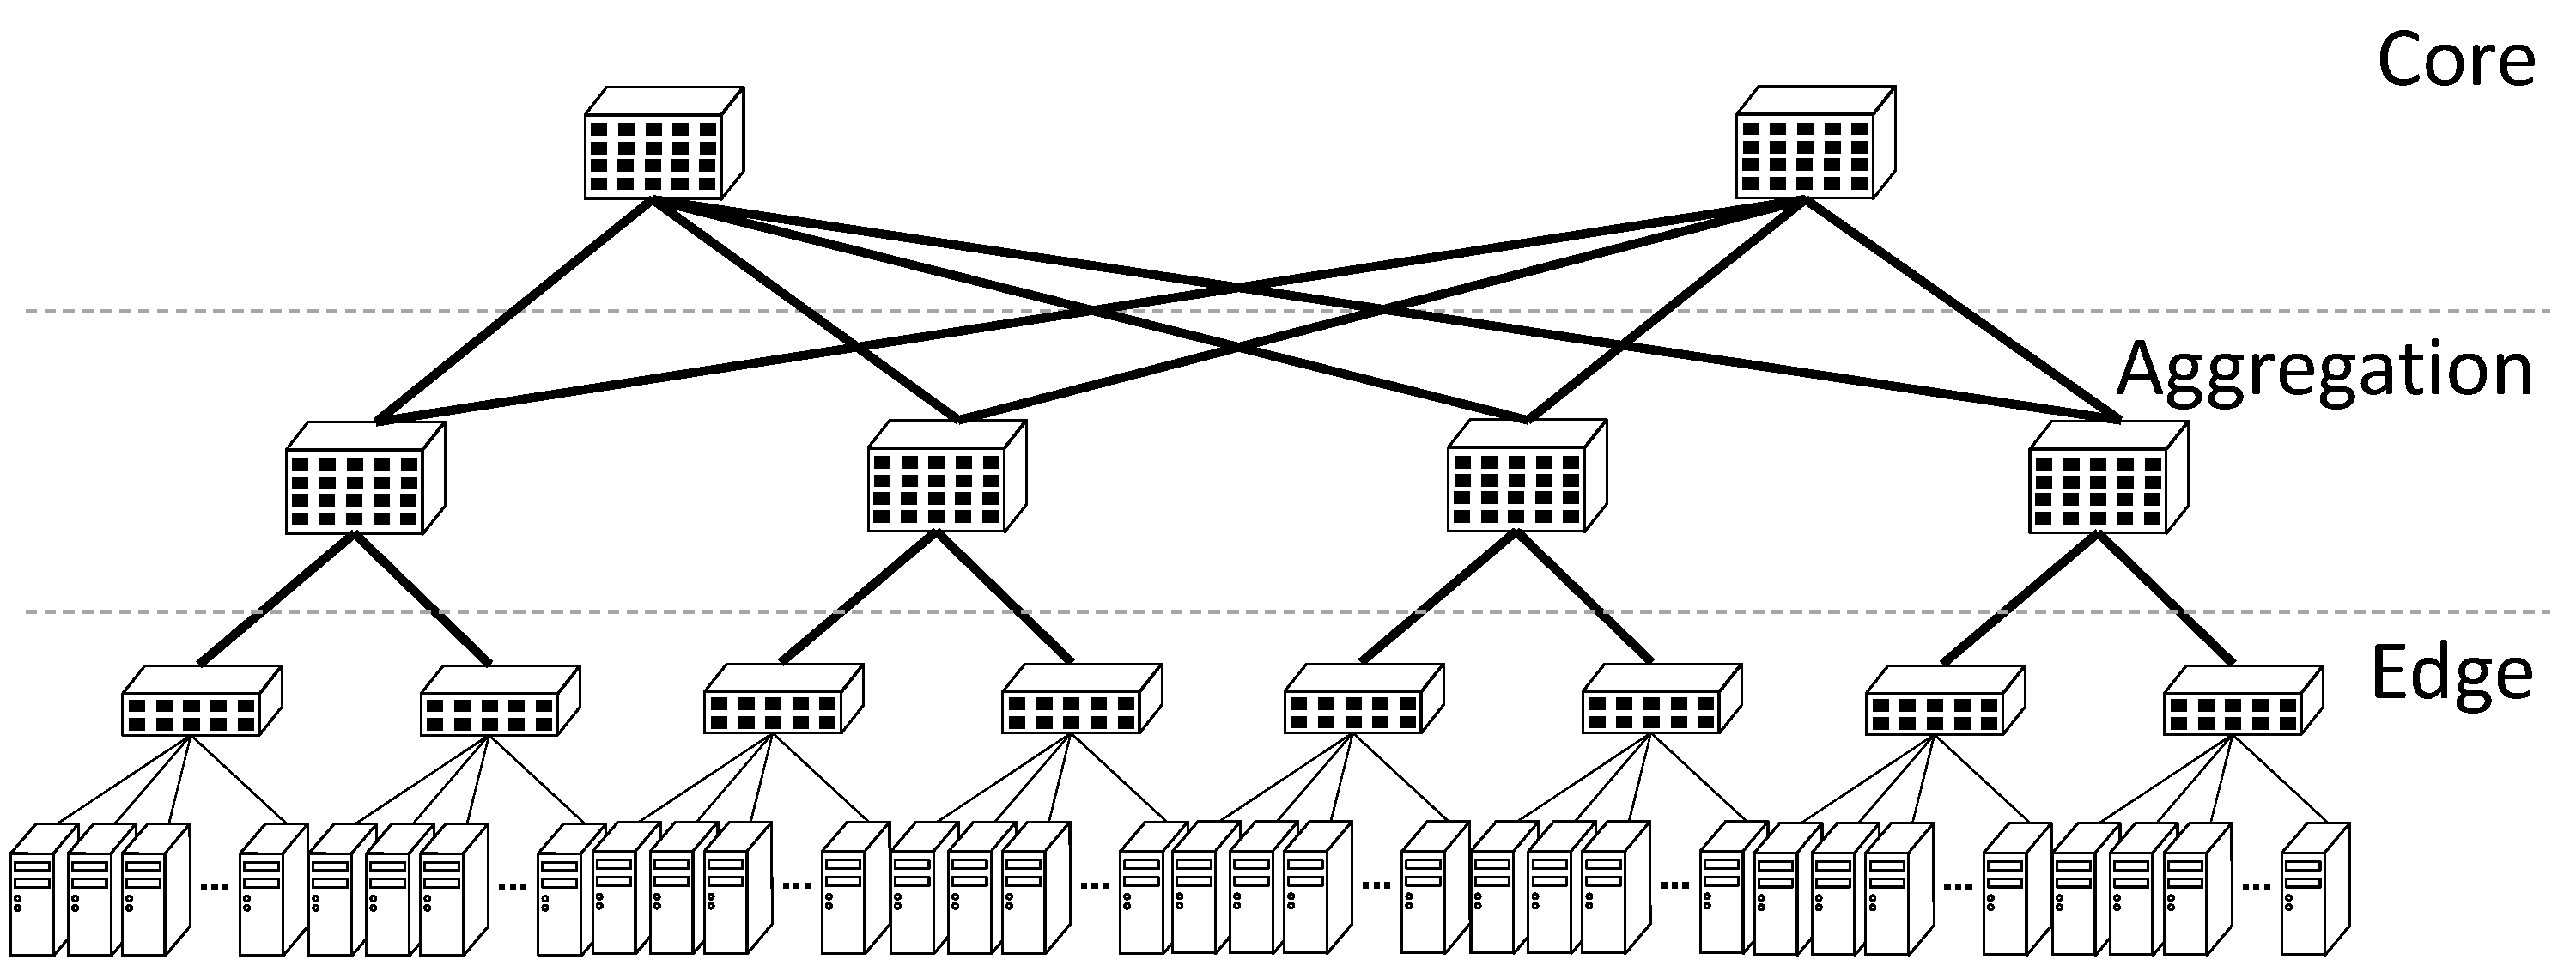
\includegraphics[width=0.35\textwidth]{conventional-hierarchical-topo}
        \label{fig:conventional_hierarchical_topo}
    }
    \\
    \vspace{-0.1in}
    \subfloat[Fat-Tree]
    {
        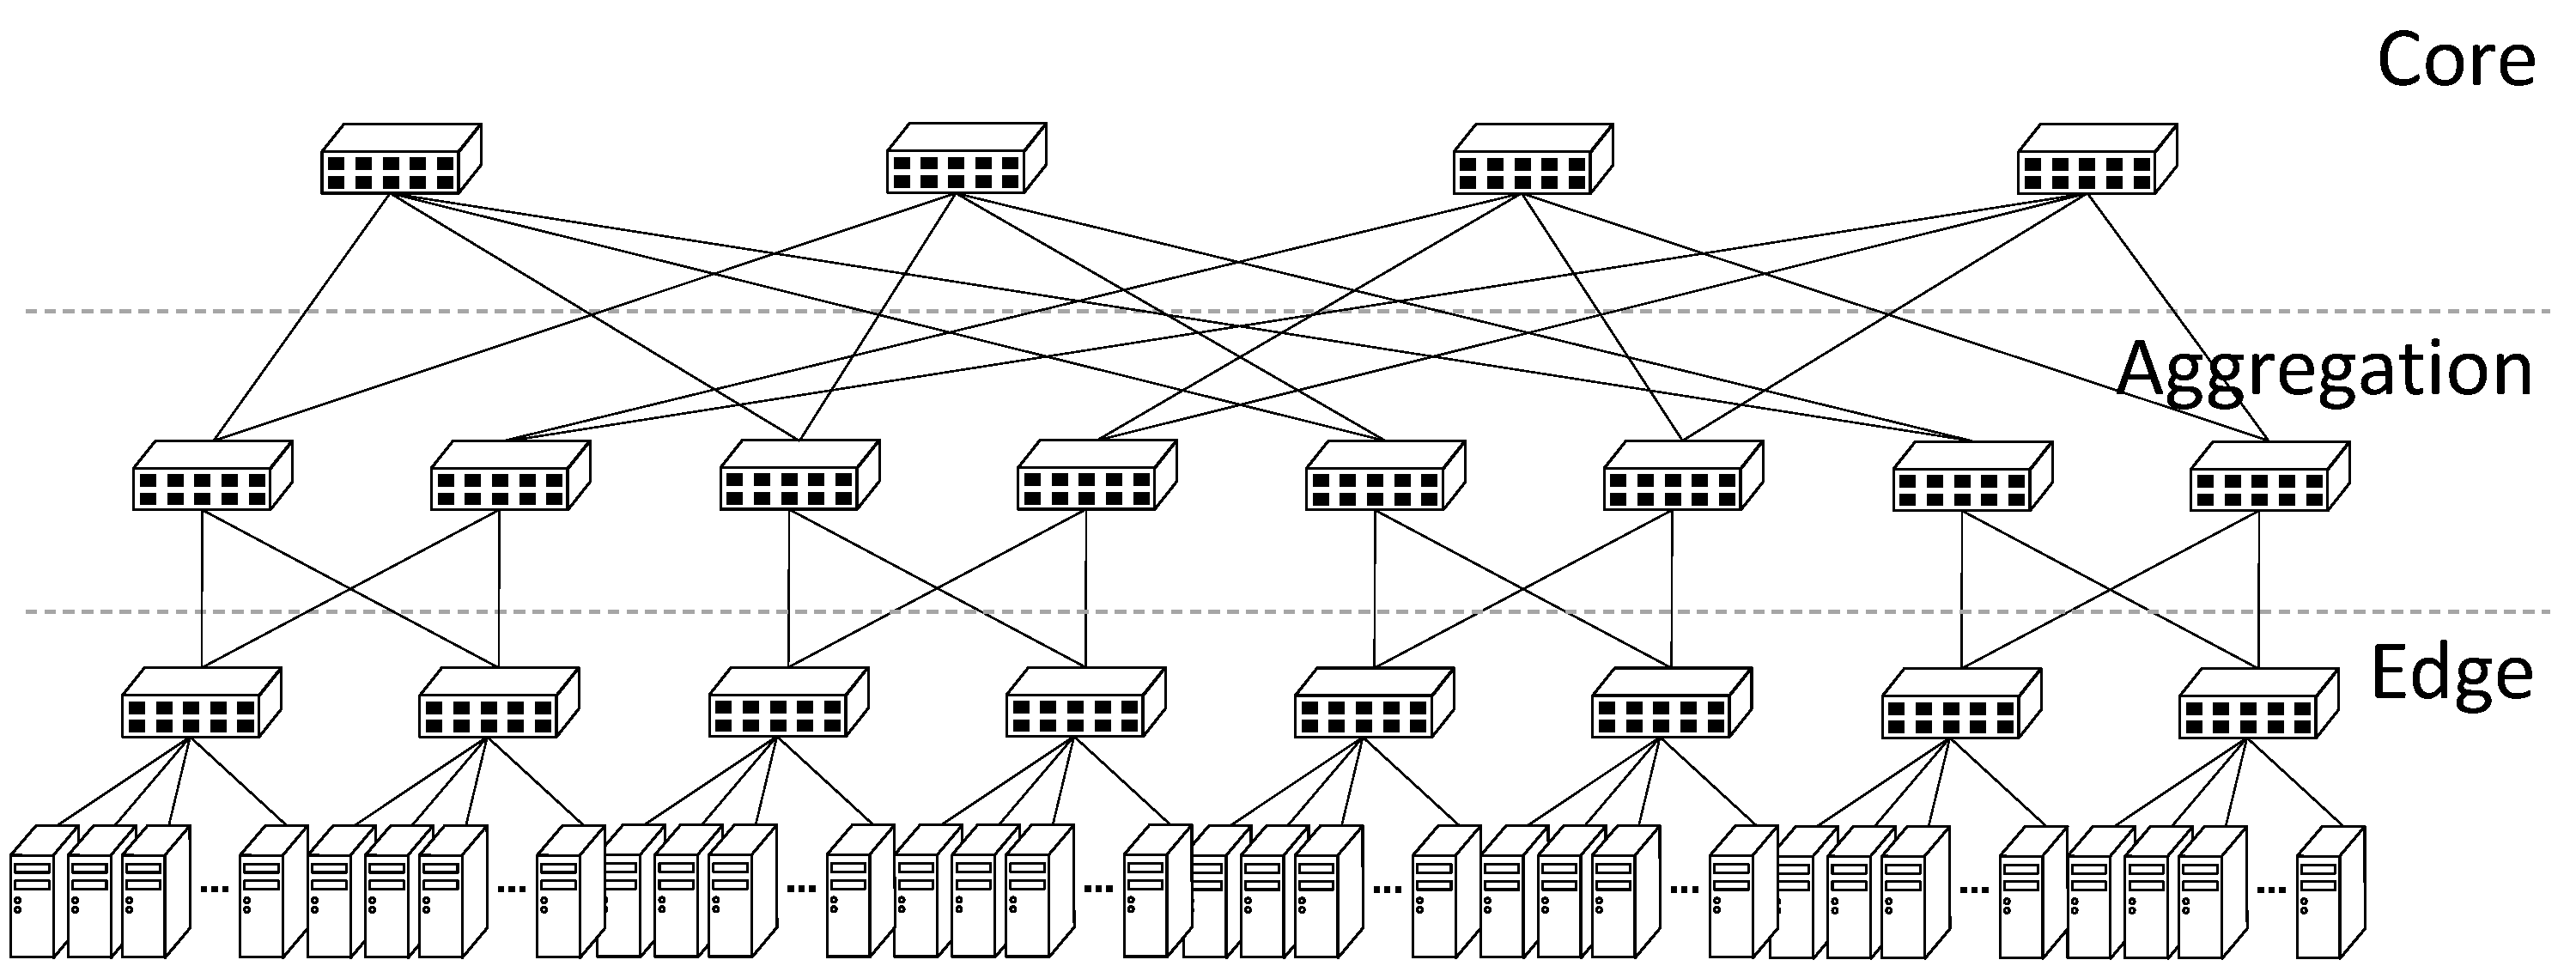
\includegraphics[width=0.35\textwidth]{fat-tree-topo}
        \label{fig:fat_tree_topo}
    }
    \vspace{-0.07in}
    \caption{Common Data Center Network Topologies}
    \vspace{-0.1in}
    \label{fig:common_topos}
\end{figure}
%\subsection {Network Stack}

Generally, the fat-tree topology is more expensive than the conventional hierarchical topology.  This is because it uses many more switches and the price difference between smaller switches and larger switches does not outweigh the difference in number of switches (see Section~\ref{sec:cost_model}).  However, the fat-tree topology provides a larger number of paths between a given source and destination, thus providing higher-bandwidth between nodes.  Having a larger number of paths between nodes also decreases the chance of network partitions since it is possible to route around failures.

\subsection {Network Stack}

Our research~\cite{Regnier:2004:TCPODCS,Alizadeh:2010:DCT,Kandula:2009:NDC} has shown that most data centers run a standard Internet stack internally consisting of Ethernet at the link layer, IP at the network layer, TCP or UDP at the transport layer, and a custom application layer protocol.  There may be special cases where proprietary protocols are used internally, however, this is uncommon.

\section{Switchless Architecture}
\label{sec:arch}
\subsection{Design}


\begin{figure}
    \centering
    \subfloat[Torus]
    {
        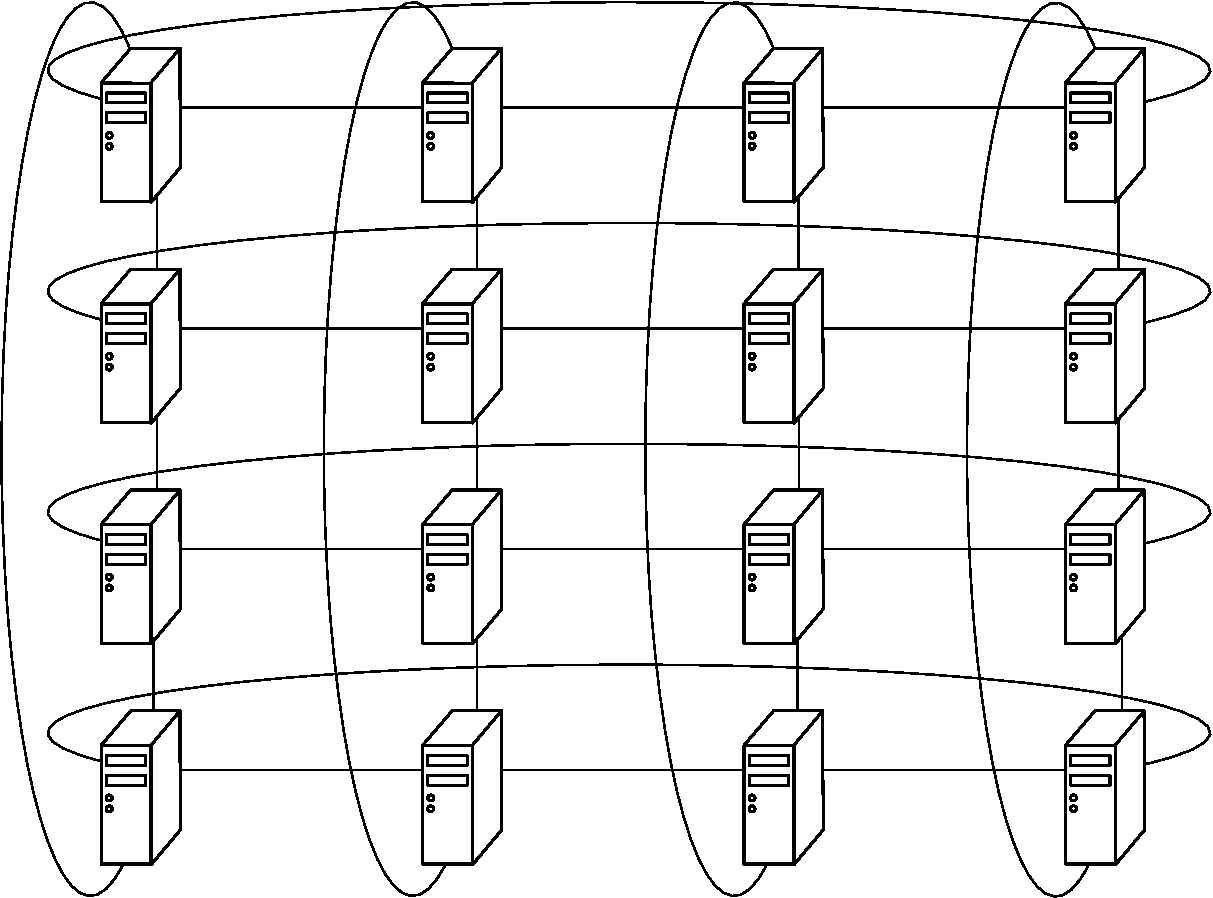
\includegraphics[width=0.3\textwidth]{switchless-arch-torus}
        \label{fig:switchless_arch_torus}
    }
    \\
    \vspace{-0.05in}
    \subfloat[Cube]
    {
        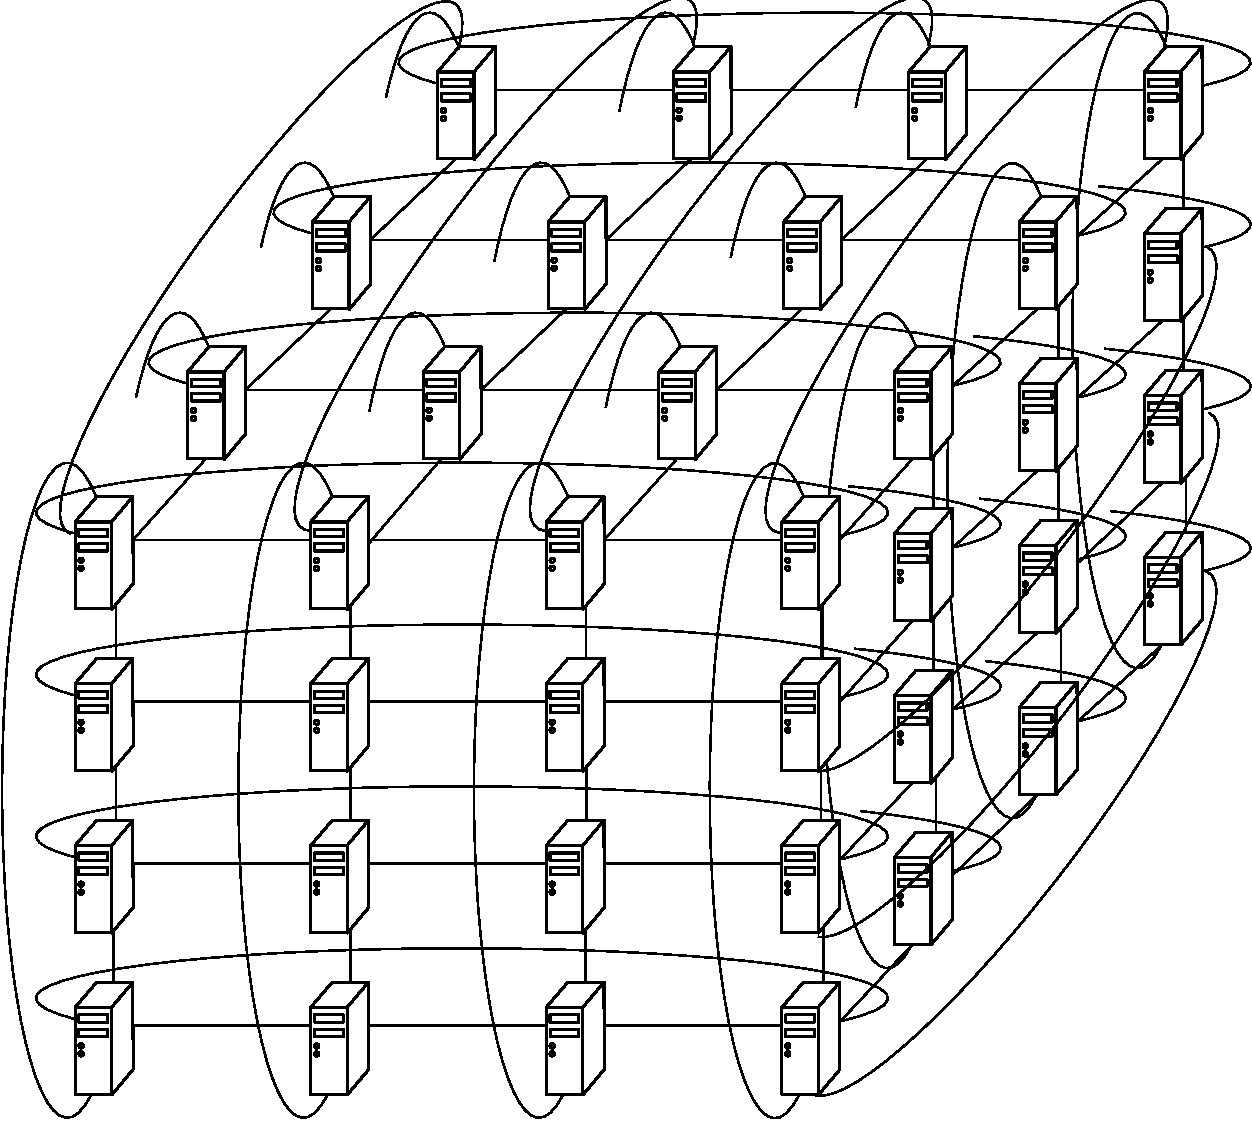
\includegraphics[width=0.3\textwidth]{switchless-arch-cube}
        \label{fig:switchless_arch_cube}
    }
    \vspace{-0.07in}
    \caption{Switchless Data Center Network Topologies}
    \label{fig:switchless_topos}
\end{figure}



Change in Topology
Removal of Switch
Change in Routing
Implementation Details
\subsection{Benefits}
Cost / Flexibility / Reliability/ Potential performance benefits (evaluated on next section)

\vspace{-0.1in}
\section{Cost Analysis}
\label{sec:cost_model}

The adoption of switchless topology in data centers will probably be driven by the low-cost of such an architecture. In this section, we attempt to predict the cost of switchless in comparison to traditional architectures like conventional hierarchical and fat-tree. As an executive summary, the overhead cost per host for switchless was calculated to be around \$70, for conventional hierarchical between \$200 and \$2000, and for fat-tree between \$10000 and \$20000.

This section is organized into two subsections. First, we will state our assumptions of commodity equipments today, how they will look in short term future, and how that affect the cost equations. Second, we provide the cost equations themselves and a graph on the overhead cost vs. number of hosts in data centers.
\vspace{-0.1in}
\subsection{Assumptions}


\subsubsection{Commercial switches}

There are two types of switches utilized in our evaluations: a top-of-rack switch that has 36 10Gbps ports plus 4 uplink 40Gbps ports, and an aggregator switch that has 32 40Gbps ports. A quick survey reveals that the current cheapest price for these are \$7k and \$14k accordingly (Mellanox SX1012 and Mellanox SX1036).

\subsubsection{Interconnects}
First, we assumed a 10Gbps Ethernet connection on all hosts and switches, with the exception of hierarchical designs where top-of-rack and aggregators are using 40Gbps links.

Second, we assume that data centers will not use copper Ethernet for links longer than 15m. While at 10Gbps, certain copper connectors are rated at up to 100m, at 40Gbps this maximum length decreases to 30m, and while there is not yet a standard for 100Gbps copper Ethernet, we would guess that these will be only able to carry clean signal at an even shorter range. Therefore, while switchless can operate solely on copper Ethernet, other topologies will have to use fiber optics at the aggregation/core range. In the following cost equations, we do not take into account the copper cost, while the fiber optic link cost is assumed to be \$1 per meter, which requires a pair of optical transceivers (10GBASE-SR or 40GBASE-SR) each costing \$200.

\subsubsection{Costs related to switchless}
Integrating a network switch on-chip will incur cost in several areas of a microprocessor. We discuss a few of these: off-chip pins, power constraint, die area consumption, and external extension board for Ethernet jacks. While there can be many sources of on-chip network switch cost, silicon cost of an additional core and an extension board cost are two huge main factors. Other sources, such as additional off-chip pins, and thermal/power related costs are negligible. 
\newcommand{\subsubsubsection}{\textbf}

\subsubsubsection{Processor pins}
We do not think that off-chip pins requirement will be a significant factor in cost due to the low number of pins required for a Ethernet connection. A standard RJ45 Ethernet jack contains 4 differential-pairs, for a total of 8 pins. With a minimum of 6 ports required for a cube switchless topology, this means we need to dedicate 48 pins to the on-chip Ethernet switch. This is only 1.5x that of 32 pins requirement for a 16x PCI-E connection, of which a regular server has up to 40x. Furthermore, it is possible for Ethernet data to be transferred through PCI-E to get to the CPU.

\subsubsubsection{Power constraint}
As estimated in~\cite{cheapsilicon}, some reasonable power consumption per-link count for a 10Gbps switch is 1W for commodity switches, 3W for programmable pipelines, and 3W for general-purpose CPU-based switches. With 6 links for a cube topology, we would expect to spend 6-18W for power consumption, depending on implementation. While we do not include power consumption in our trade-off analysis, heat dissipation limit of the CPU is a major limitation on potential switchless architectures.

\subsubsubsection{Die area cost}
Die area cost of an on-chip switch is hugely dependent on the implementation, and the switching features needed. Here we will only give a bare minimum estimation.

The most favorable scenario for a minimum implementation is when we can have a custom routing protocol, like the dimension-ordered L3 protocol described in Section~\ref{sec:arch:sec:net_stack}. This implementation mirrors a router in a NoC: each host has its own unique XYZ coordinate, and a routing decision can be trivially made with a dimension comparison.

However, the same can be said for fat-tree or hierarchical topologies where a custom protocol can hugely improve performance and implementation cost. Instead, commercial switches need to adhere to standards like TCP, IP, and Ethernet, which complicate implementation. Assuming that we want our on-chip switch to be MAC address compatible, we would need to keep a MAC table big enough to store all the MACs in the immediate network. It turns out that such a 16k-entry table would be around 100KB in size. Furthermore, this table will need to be implemented as a hash-table, as CAMing a 16k-entry table is not feasible.

In the worst case, a dedicated CPU core is needed to manage the hash table. Now we have a different question: whether a single core is fast enough to switch packets without performance degradation. It turns out that, for 1500B packets and 10Gbps, an Ethernet link will interrupt the processor 833 times a second. A single RISC core at 2GHz will have ample time to multiplex multiple links.

Considering the cost of such a processor in products like Beaglebone, we estimate the silicon cost of an additional dedicated core at \$20 for calculation purposes.

\subsubsubsection{Extension board}
Hosts' motherboards will probably not have 6 Ethernet jacks to be used for switchless, so we include an extension board to the cost equation at \$50 per host.
\vspace{-0.1in}
\subsection{Cost model equations}
The general formula has three parts: the cost of switches, cost of interconnect (fiber optics), and other costs. This cost is "per-host".
\vspace{-0.1in}
\begin{multline}
Cost = Switch_{cost} + Interconnect_{cost} + Other_{cost}
\end{multline}
\subsubsection{Hierarchical}
In hierarchical topologies, we have three types of switches:
\vspace{-0.1in}
\begin{multline}
Switch_{cost} = ToR_{cost} + Agg_{cost} + Core_{cost}
\end{multline}
Top-of-rack switches are the low-end ones with 10Gbps connections to the hosts, and aggragators and core switches are assumed to be the same kind with 40Gbps ports.
\vspace{-0.1in}
\begin{multline}
Switch_{cost} = \$7000 * ToR_n +\\
                \$14000 * (Agg_n + Core_n)
\end{multline}
We assume that fiber optics are used to connect ToR, Agg, and Core together. The cost below includes the transceivers which cost \$200 each.
\vspace{-0.1in}
\begin{multline}
Interconnect_{cost} = \$450 * (ToR_n * Agg_n) +\\
                      \$500 * (Agg_n * Core_n)
\end{multline}
\subsubsection{Fat-tree}
The basic fat-tree for Ethernet as proposed in~\ref{fat-tree} has a $k$ parameter that dictates how many host the topology can support. It also utilizes only one type of switches. Fiber optics are assumed to be used between aggregation and core switches.
\vspace{-0.1in}
\begin{align}
Switch_{cost} = \$7000 * (K^2 + K^2 / 4) \\
Interconnect_{cost} = \$500 * (K^4 / 8)
\end{align}
\subsubsection{Switchless}
Switchless does not have switches, and we do not take into acount the copper Ethernet cables. Its other costs involve the cost of silicon (\$20) and the cost of the extension board (\$50).

\subsection{Analysis}

\captionsetup[subfloat]{captionskip=-0.003in}
\begin{figure}
    \centering
    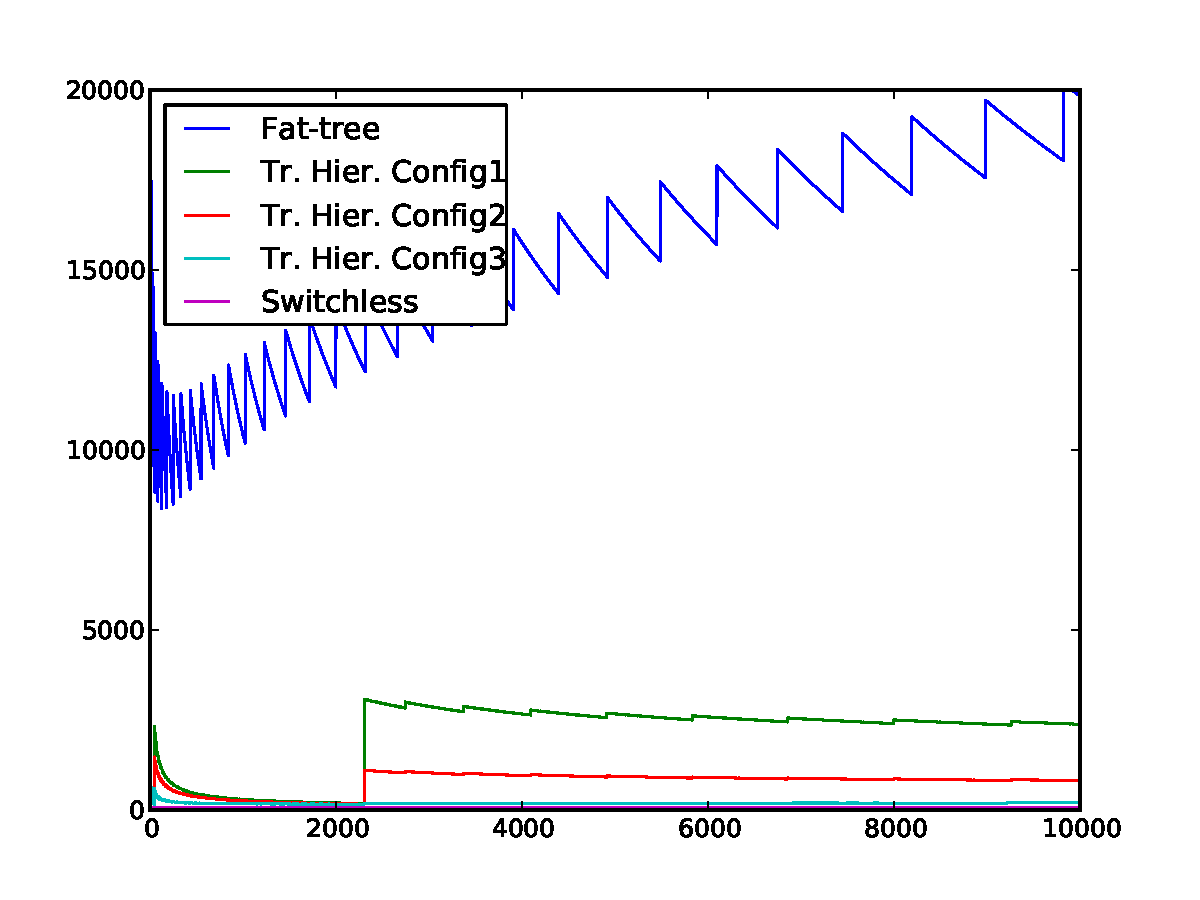
\includegraphics[width=0.3\textwidth]{10000_linear_permachinecost}
    \vspace{-0.1in}
    \caption{Per-host cost of network as number of host is increased to 10,000.}
    \label{fig:cost_perhost}
\end{figure}

As seen in Figure~\ref{fig:cost_perhost}, the cost of fat-tree can increase up to \$20000, traditional hierarchy (with bandwidth overprovisioning) to \$2000, while switchless remains a flat \$70.


\vspace{-0.1in}
\section{Evaluation}
\label{sec:eval}
In this paper, we attempt to address performance concerns in the switchless architecture: how does the performance compare when running a workload like weather modeling or Apache's Hadoop[CITE]? To this end, we simulate a micro-benchmark with parameters that approximate real workloads on two switchless topologies (torus and cube), and two traditional topologies (fat-tree and hierarchical). As alluded to in Section~\ref{sec:arch}, we do not expect switchless to have higher performance than a fat-tree on all applications. Yet, with the massive force of low-cost attached to switchless, we would hope that any performance degradation would be acceptable.

%We also ran a few more benchmarks such as a bandwidth stress test to see the effect of increasing data transfer rate, as well as the efficiency of UDP vs TCP.
We also ran other simulations to compare the overhead of UDP versus TCP in the data center setting, as well as IP routing versus dimension-ordered routing.

\subsection {Methodology}
For performance evaluation, we use the ns-3 simulator\cite{Ns3:Online}, an open-source discrete-event network simulator developed by the networking research community[CITE]. We modified a significant portion of the simulator for our purpose. These modifications include adding a dimension ordered routing protocol, creating various network topologies for both switchless and conventional architectures, and constructing a highly configurable synthetic micro-benchmark.  Due to time constraints, we did not modify ns-3 to implement wormhole routing and do not make any claims about it in our evaluation.  The ns-3 simulator, augmented with our modifications, models all five OSI stack layers.

As it is hard to define a small representative application for the data center, we used a synthetic micro-benchmark that can be configured to model various application's communication pattern. For example, this micro-benchmark can be configured to generate simple all-to-all style communication traffic with certain intensity. On the other hand, it can also be configured to generate sporadic communications between two random nodes. Note that there are many other possible configurations which create different communication patterns for modeling application communication patterns.

% benchmark configurations (common)
The default configurations for all simulations are detailed in Table~\ref{tab:configurations}, unless noted specifically.  All switchless topologies (torus and cube) use dimension ordered routing, while all traditional topologies (conventional hierarchy and fat-tree) use IP routing.
% # host: 512
% Ethernet links: 1Gbps
% hierarchical: 1 core, balanced fan-outs (agg / edge == edge / host)
% link/switching latency is 500ns for all topologies!!!!!!!!!!! (might be wrong)
% cube z-dimension limit is 40
% all topologies are running on UDP
% switchless are using dimension ordered routing
% 4KB packet length

\subsection {Results}
% Results -- 
% (1) Impact of topology change on performance
% (2) Impact of routing change on performance
% (3) Application Sensitivity (Different application configurations)
% (4) Scalability (host count change)


\subsubsection{N-Body simulation performance}
\newcommand{\nbody}{N-Body}
In a classic \nbody~simulation, all nodes communicate to all other nodes. Figure~\ref{fig:nbody_packetdelay} shows the packet delay distribution of all packets sent in one computation round of an \nbody~simulation for all topologies and network stacks; Figure~\ref{fig:nbody_latency} shows the longest packet delay--the global communication latency of a computation round--compared.

\captionsetup[subfloat]{captionskip=-0.003in}
\begin{figure}
    \centering
    \subfloat[Packet Delay Distribution]
    {
        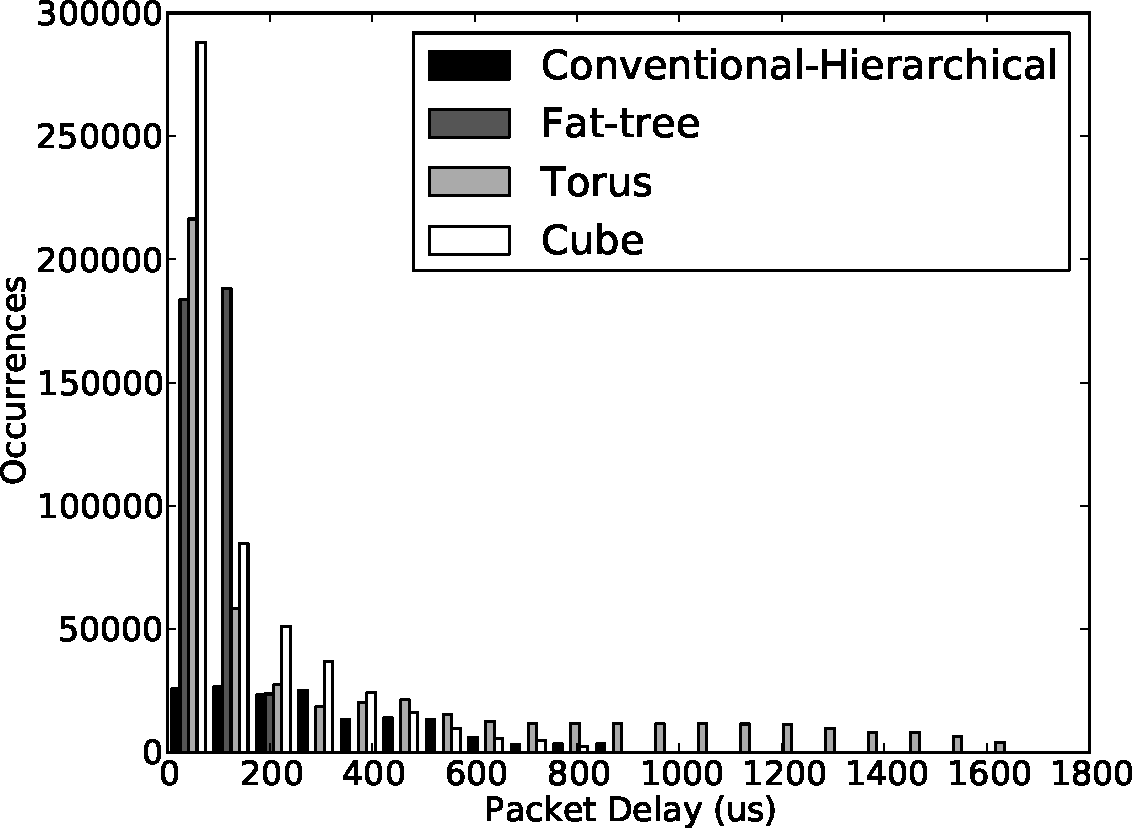
\includegraphics[width=0.3\textwidth]{nbody_delay}
        \label{fig:nbody_packetdelay}
    }
    \\
    \vspace{-0.1in}
    \subfloat[Longest Delay]
    {
        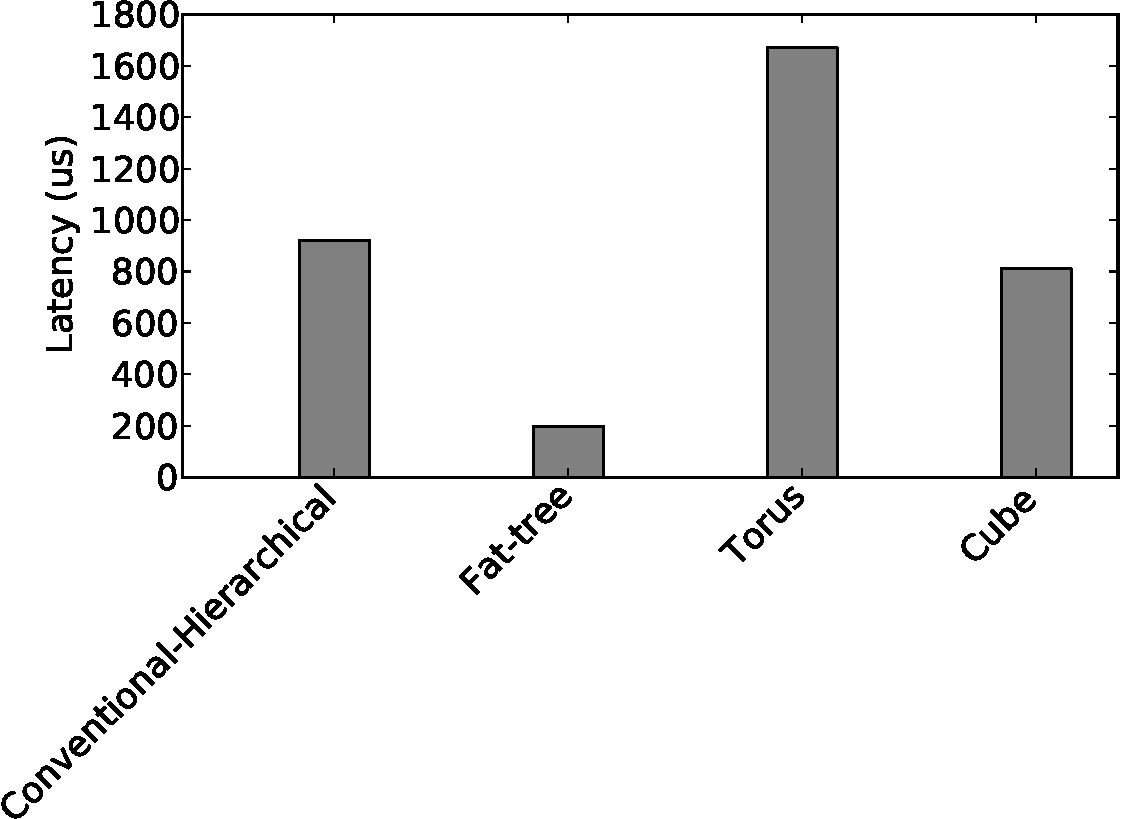
\includegraphics[width=0.3\textwidth]{nbody_latency.pdf}
        \label{fig:nbody_latency}
    }
    \vspace{-0.07in}
    \caption{N-Body Simulation Results}
    \label{fig:common_topos}
\end{figure}

While switchless topologies have higher occurrences of short packet delay (nodes close together), there are also a smaller number of packets with long delays (nodes far away) that limit the global computation throughput of an \nbody simulation. As shown in Figure~\ref{fig:nbody_latency}, fat-tree is about four times faster than cube and conventional hierarchy, and as much as seven times faster than the torus topology.

On the other hand, it does not necessarily mean that simulation under fat-tree is 4 times faster than cube: the computational time is needed to compute overall performance. [IS THIS TRUE]??
% perhaps we need a plot here, comparing different topologies' time in y axis with computational time in the x axis.

\subsubsection{Weather modeling performance}
In weather modeling, every node communicates with only its neighbors; this means that every node in the system communicates to six other nodes in the cube topology. This workload should map very well to switchless topologies, whereas hierarchical and fat-tree could still perform well but the energy cost may be significant. [WHAT DOES NEIGHBORS MEAN FOR HIERARCHICAL AND FAT-TREE??]

\captionsetup[subfloat]{captionskip=-0.003in}
\begin{figure}
    \centering
    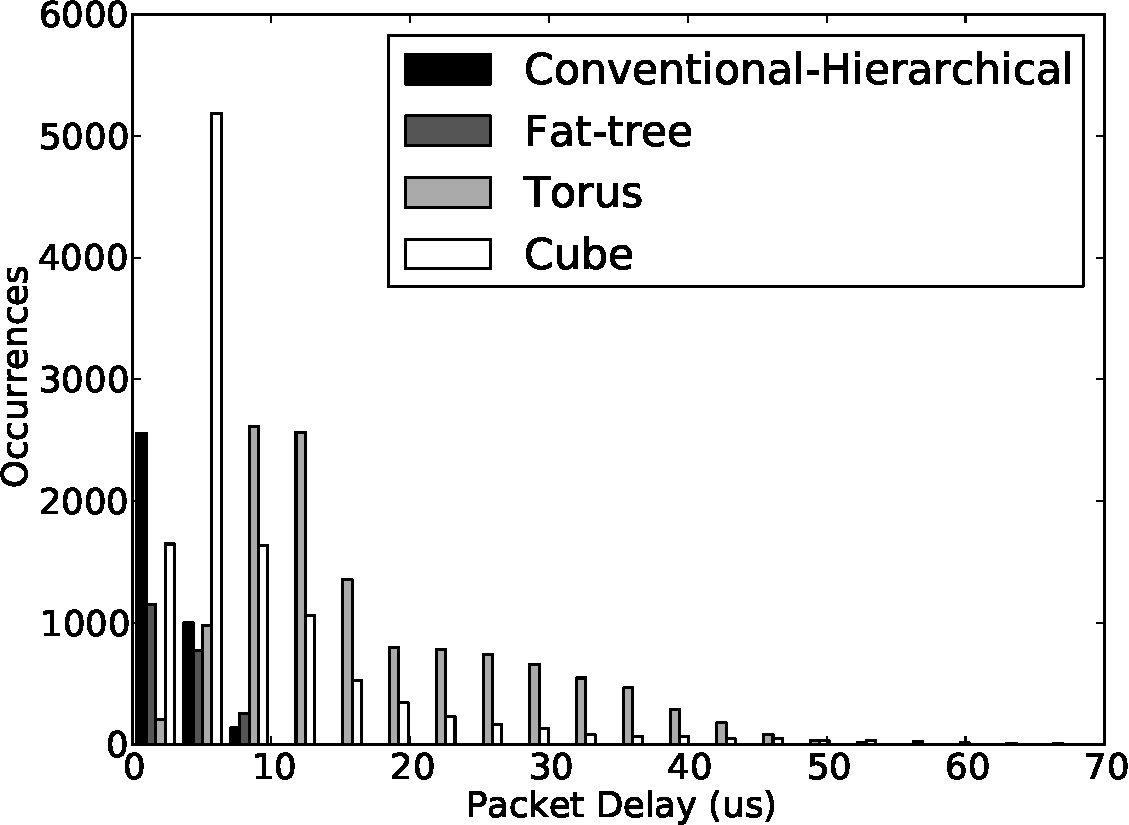
\includegraphics[width=0.3\textwidth]{weather_delay}    
    \vspace{-0.1in}
    \caption{Weather Modeling Packet Delay Distribution}
    \label{fig:weather_packetdelay}
\end{figure}

Figure~\ref{fig:weather_packetdelay} shows the distribution graph of all packets transferred in a computation round of a weather modeling simulation with six neighbors. For a reason not quite understood, a long tail can still be seen with both cube and torus topology. [WE SHOULD UNDERSTAND THIS OR GIVE SOME REASONS, I HAVE SOME IDEAS]

On the other hand, there are a few reasons why hierarchical or fat-tree has good performance. The most conspicuous reason is that our micro-benchmark doesn't map exactly to a weather modeling simulation in that for each node we pick the six closest neighbors, which will always be in the same rack [IS THIS TRUE???]. If time allows, we will adjust the parameters for a more accurate results.

\subsubsection{Random N to random M}

\captionsetup[subfloat]{captionskip=-0.003in}
\begin{figure}
    \centering
    \subfloat[Packet Delay Distribution]
    {
        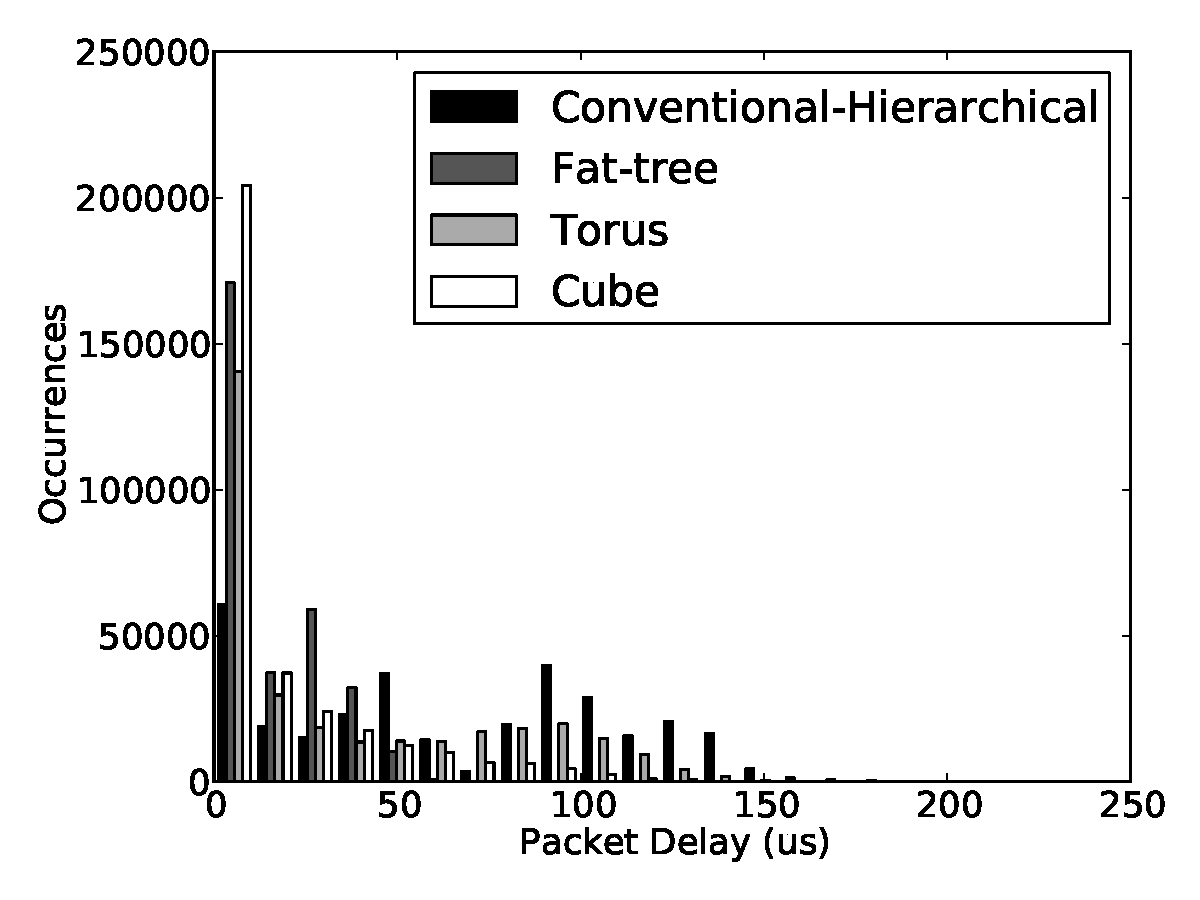
\includegraphics[width=0.3\textwidth]{25_delay}
        \label{fig:25_packetdelay}
    }
    \\
    \vspace{-0.1in}
    \subfloat[Longest Delay]
    {
        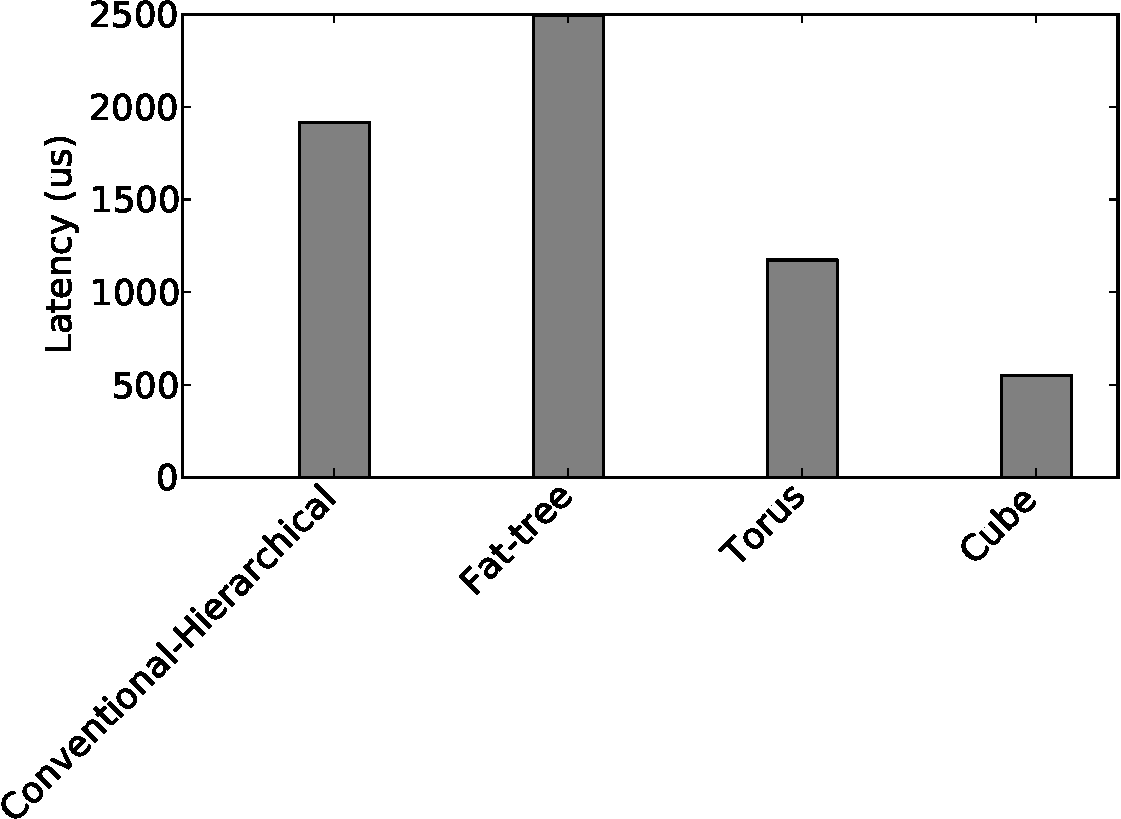
\includegraphics[width=0.3\textwidth]{25_latency.pdf}
        \label{fig:25_latency}
    }
    \vspace{-0.07in}
    \caption{RNRM Simulation Results}
\end{figure}


\subsubsection{TCP vs UDP}
Data center operators usually run TCP as the level 4 networking stack for better compatibility with MAN and WAN [CITE?? I DONT THINK THIS IS TRUE]. However, TCP has more overhead compared with UDP, and TCP guarantees are not necessary in data centers where dropped packet are rare. As we utilize a full network stack simulator for our study, we implement our topologies with both TCP and UDP and run a simulation exercise to see how the overheads compare.

What we found was that, at least for our simulation set up, TCP has about the same performance as UDP, but packet drops are more frequent, leading to completion time timing out.


\subsubsection{Dimension-ordered vs IP}
As mentioned, for switchless topologies, we had two implementations: one with TCP/IP routing, and the other one with dimension-ordered routing commonly used in NoC for deadlock avoidance. In our simulation, as shown in Figure~\ref{fig:dim_ordered}, we found that for some reason dimension-ordered routing is slower than IP. One possible reason for this is that dimension-ordered protocol restricts the possible data paths that packet can traverse through, and so introduces bandwidth contentions that otherwise might not exist in traditional IP routing.

\captionsetup[subfloat]{captionskip=-0.003in}
\begin{figure}
    \centering
    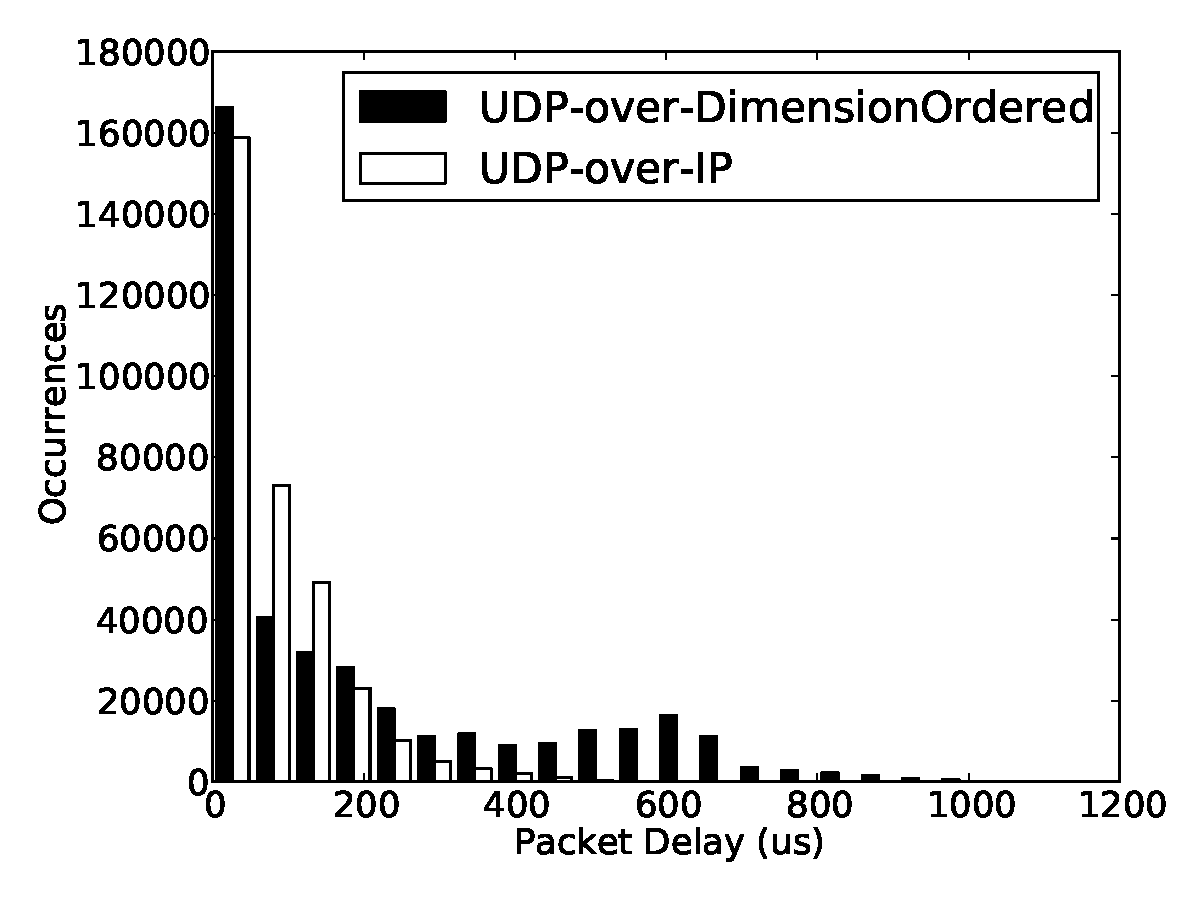
\includegraphics[width=0.3\textwidth]{dimension_ordered_udp}
    \vspace{-0.1in}
    \caption{Packet Delay Distribution of a Torus Network Running UDP Over IP and UDP Over Dimension Ordered.}
    \label{fig:dim_ordered}
\end{figure}


\vspace{-0.1in}
\section{Related Work}
\label{sec:related}

While interconnection network has been a popular topic in the community for a long time\cite{datacenter3}, only few recent literatures introduce network architectures that are suited for data center usage. Representative literature suggests some specific data center network architectures or topologies such as fat-tree \cite{Al-Fares:2008:SCD, datacenter4}, DCell\cite{datacenter2}, and BCube\cite{datacenter5}. 

Fat-tree suffers from high-cost problem because it requires large, high-performance switches and expensive fiber optic inter-switch links. BCube and DCell uses fewer switches and inter-switch links but still has the high cost. While those previously proposed data center network architectures are soley focusing on performance optimization, our data center network architecture focuses on both performance and cost per performance. In addition, our switchless network architecture also offers other qualitative benefits mentioned in earlier part of this paper.
\vspace{-0.1in}
\section{Conclusions}
\label{sec:conclusion}
In this work, we proposed an economic alternative of the conventional data center network architecture : switchless network architecture. Our analysis and evaluation show that our switchless network architecture can deliver comparable performance at a much lower cost thereby having much better cost per performance. 

\newpage
%% Bibliography
%\vspace{-1ex}
%\linespread{1.0}
%\setlength{\bibsep}{1pt}
%\footnotesize
\small
\bibliography{local}
\bibliographystyle{abbrvnat}

\end{document}

